\documentclass[twoside,11pt]{article}

\usepackage{aa228-jmlr2e}
\usepackage{lipsum}
\usepackage{listings}

\input{julia_listing}

\begin{document}

% Refer to this link for project rubric: https://aa228.stanford.edu/project-1/
\title{Project 1: Bayesian Structure Learning}

%===========================================
% TODO: Replace "First Last" with your name.
% TODO: Replace "email@stanford.edu" with your Stanford email.
%===========================================
\name{Christopher Luey}
\email{luey@stanford.edu}


\maketitle

\section{Algorithm Description}
%===========================================
% TODO: Replace this with a short description of your algorithm(s) used.
This project implements a comprehensive Bayesian network structure learning system that combines multiple search heuristics to maximize the Bayesian Dirichlet equivalent uniform (BDeu) score with a Dirichlet(1) prior. The implementation uses an ensemble approach where three distinct algorithms are run sequentially, each seeded with the best results from prior searches.

The core scoring mechanism uses the BDeu metric with uniform Dirichlet prior ($\alpha_{ijk} = 1$). To improve scalability, the implementation employs mutual information-based parent candidate selection, reducing the search space from $O(n^2)$ to $O(nk)$ without significantly impacting solution quality.

The multi-algorithm ensemble consists of: (1) Hill Climbing with Tabu Search using greedy hill climbing with multiple random restarts and tabu memory to escape local optima, (2) Simulated Annealing using Metropolis-Hastings sampling with exponential temperature cooling to allow temporary moves to lower-scoring regions, and (3) Genetic Algorithm using edge-recombination with tournament selection, crossover, and mutation operators, seeded with the best solutions from previous phases.

The DAG representation uses adjacency matrices with efficient cycle detection via depth-first reachability checks. All local scores are maintained incrementally, avoiding redundant re-computation. The system automatically scales hyperparameters based on problem size.
%===========================================


\section{Graphs}
%===========================================
% TODO: Add your small, medium, and large graph visualizations here
%===========================================
\begin{figure}[h]
    \centering
    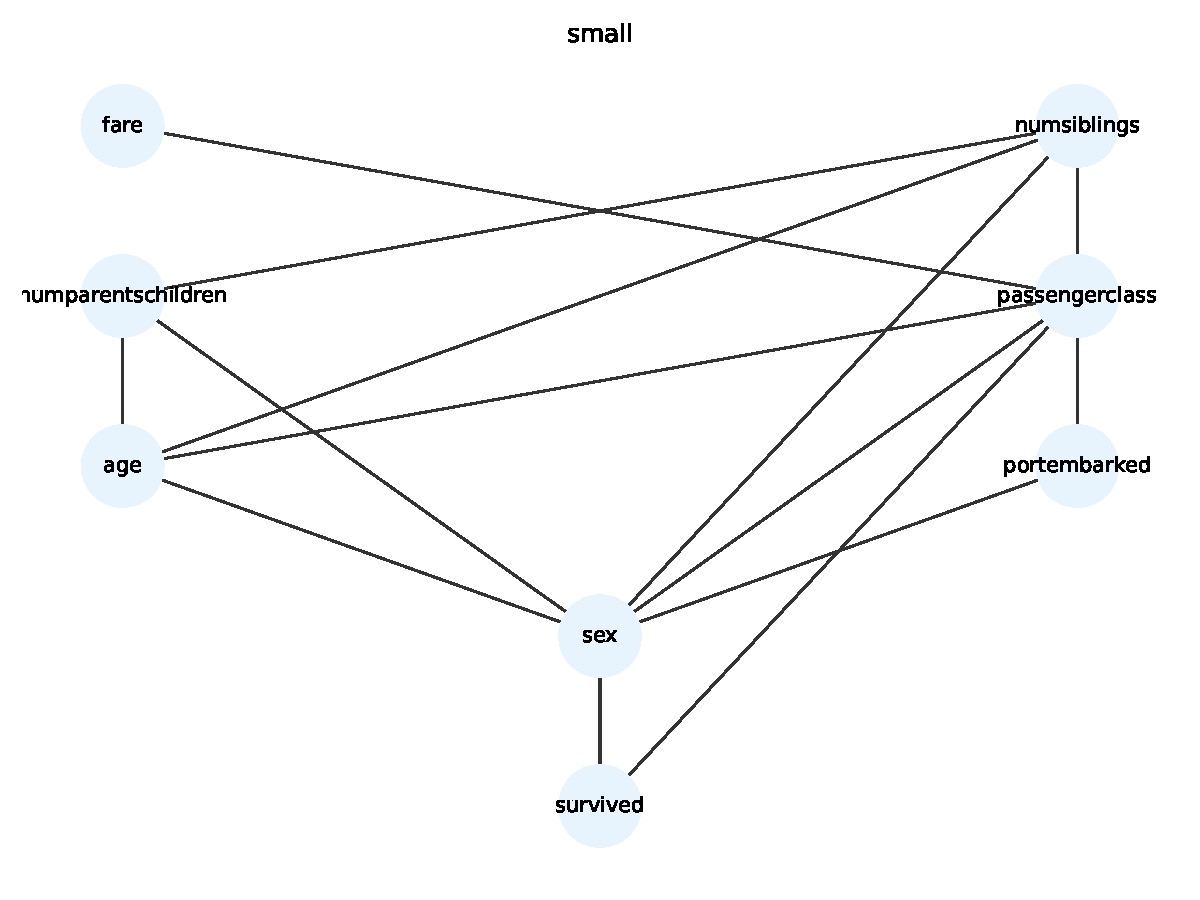
\includegraphics[width=0.7\textwidth]{small_graph.pdf}
    \caption{Bayesian network learned from the Titanic dataset (889 rows, 8 variables, 14 edges). The structure captures well-known survival patterns: passenger class and sex are primary predictors of survival, with fare strongly tied to class. Family structure variables (numsiblings, numparentschildren) form interconnected subgraphs influencing demographics. Score: $-3794.86$ (genetic algorithm). Runtime: 2.6 seconds.}
\end{figure}

\begin{figure}[h]
    \centering
    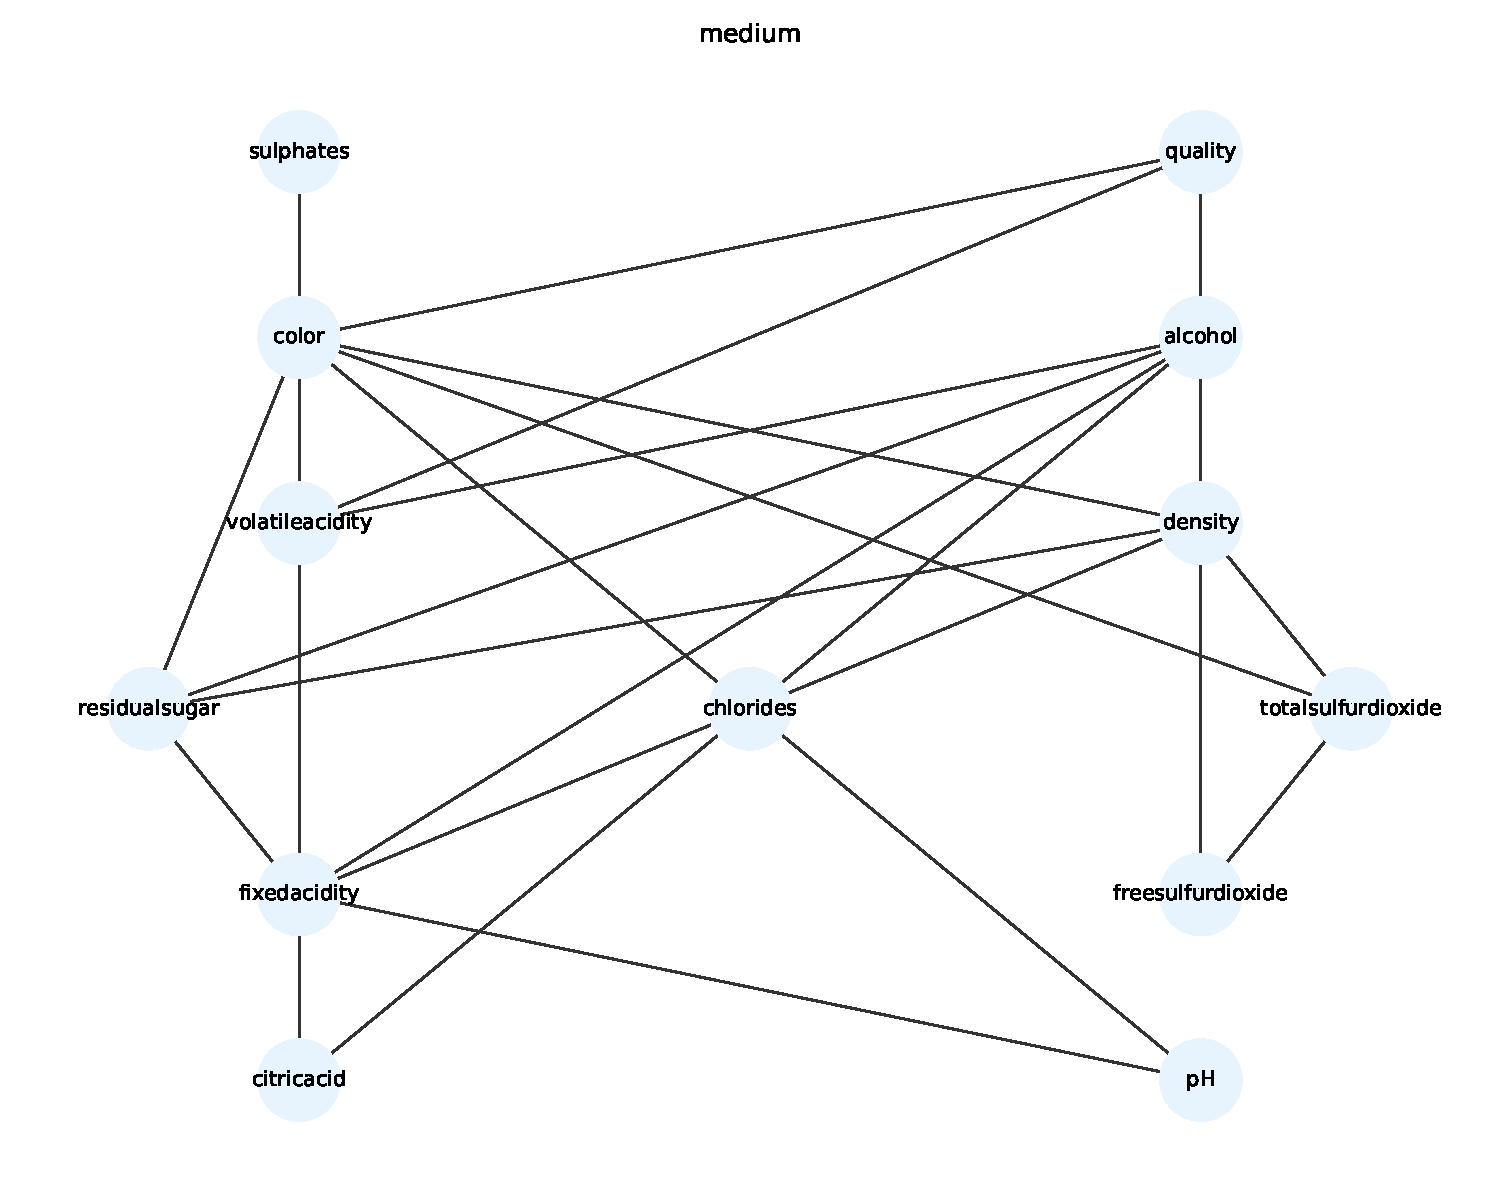
\includegraphics[width=0.85\textwidth]{medium_graph.pdf}
    \caption{Bayesian network learned from the wine quality dataset (6497 rows, 13 variables, 28 edges). Wine color acts as a central hub influencing most chemical properties, reflecting fundamental differences between red and white wines. Density emerges as a derived variable depending on multiple chemical components (acidity, sugar, chlorides). Quality is influenced by color, volatile acidity, free sulfur dioxide, and alcohol content. Score: $-96312.06$ (genetic algorithm). Runtime: 5.7 minutes.}
\end{figure}

\begin{figure}[h]
    \centering
    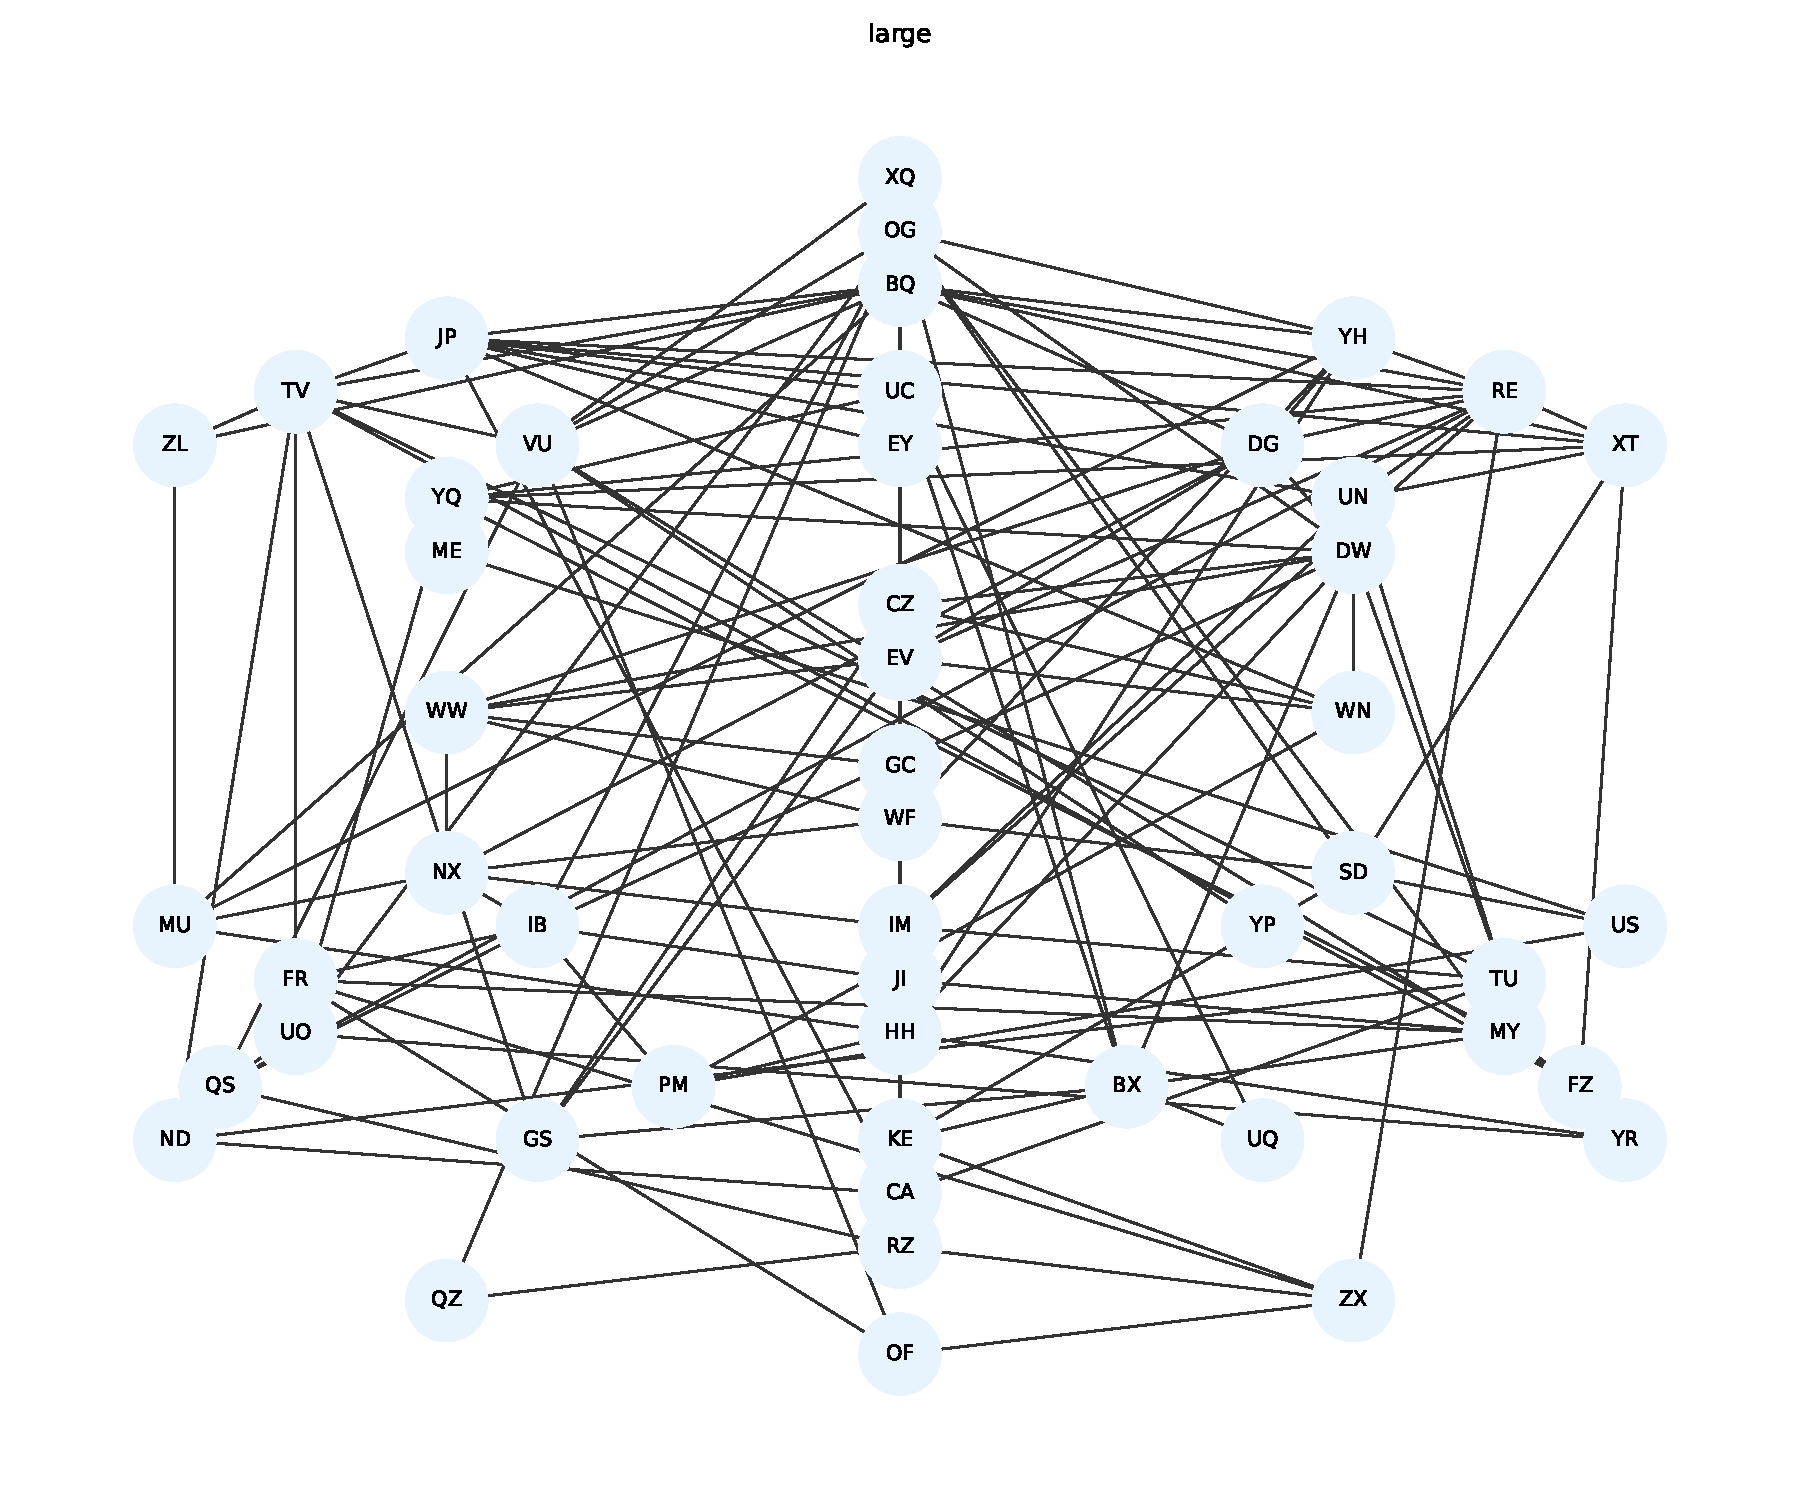
\includegraphics[width=0.95\textwidth]{large_graph.pdf}
    \caption{Bayesian network learned from a large synthetic dataset (10000 rows, 50 variables, 138 edges). The learned structure is highly interconnected, with an average of 2.76 edges per variable. Several variables act as hub nodes with high in-degree or out-degree, suggesting latent cluster structure in the synthetic generation process. The genetic algorithm achieved a score of $-420800.40$, outperforming both hill climbing ($-422299.66$) and simulated annealing by nearly 1500 log-score units. Runtime: 3.9 minutes.}
\end{figure}


\section{Code}
%===========================================
% TODO: Add your code here, see code listing options here: https://www.overleaf.com/learn/latex/code_listing
% NOTE: Code does not count towards your page limit!
% OPTIONS:
%   1. Paste everything into a {verbatim} environment (where all characters are parsed...verbatim).
%   or 2. paste everything into a {lstlisting} environment for syntax highlighting (examples for Julia and Python below).
% NOTE: Feel free to break up functions into separate {algorithm} + {lstlisting} environments for better organization (not required!) 
%===========================================

The complete implementation is available in the attached \texttt{project1.py} file. The main components include:

\begin{algorithm}
\begin{lstlisting}[language=Python]
import argparse
import sys
from pathlib import Path
from typing import Dict, List, Tuple

from structure_learning import (
    DiscreteDataset,
    StructureLearner,
    default_config,
)

def write_gph(edges: List[Tuple[int, int]], idx2names: Dict[int, str], filename: str) -> None:
    """Write graph edges to .gph file in required format."""
    out_path = Path(filename)
    out_path.parent.mkdir(parents=True, exist_ok=True)
    with out_path.open("w") as fh:
        for u, v in edges:
            fh.write(f"{idx2names[u]}, {idx2names[v]}\n")

def compute(infile: str, outfile: str) -> None:
    """Main computation: load data, learn structure, write results."""
    # Load dataset
    dataset = DiscreteDataset(infile)
    
    # Generate configuration
    config = default_config(dataset.num_vars, dataset.num_rows)
    
    # Run structure learning
    learner = StructureLearner(dataset, config)
    result = learner.learn()
    
    # Write output
    edges = list(result.dag.edges())
    idx2name = {idx: name for idx, name in enumerate(dataset.names)}
    write_gph(edges, idx2name, outfile)

def main(argv: List[str] | None = None) -> None:
    """CLI entry point."""
    parser = argparse.ArgumentParser(description="Bayesian structure learning")
    parser.add_argument("input_csv", help="Input CSV file")
    parser.add_argument("output_gph", help="Output .gph file")
    args = parser.parse_args(sys.argv[1:] if argv is None else argv)
    
    compute(args.input_csv, args.output_gph)

if __name__ == "__main__":
    main()
\end{lstlisting}
\end{algorithm}

The core structure learning algorithms are implemented in \texttt{structure\_learning.py}, which includes:
\begin{itemize}
\item \texttt{DiscreteDataset}: Data loading and preprocessing
\item \texttt{BDeuScoreCache}: Efficient score computation and caching
\item \texttt{DAG}: Graph representation with cycle detection
\item \texttt{HillClimber}: Hill climbing with tabu search
\item \texttt{SimulatedAnnealing}: Metropolis-Hastings sampling
\item \texttt{GeneticAlgorithm}: Edge-recombination genetic algorithm
\item \texttt{StructureLearner}: Orchestrates the ensemble approach
\end{itemize}

\end{document}
